% Crucial Preamble
\documentclass[12pt,letterpaper]{article} \usepackage{amsmath} \usepackage{graphicx} \usepackage[margin=1in]{geometry} \usepackage{longtable}  \usepackage{amssymb}

% Extra Preamble
\usepackage{fancyhdr} \usepackage{enumitem} \usepackage{float} \usepackage{soul}
\usepackage{multicol} \usepackage[compact]{titlesec}


% frames with display breaks
\usepackage{mdframed}
\allowdisplaybreaks

% change spacing
\usepackage{setspace}
\setlength{\parskip}{0.4\baselineskip}

% Remove paragraph indentation
\setlength{\parindent}{0pt}

% Reduce space before and after section headings
%\titlespacing*{\section}{0pt}{0.1\baselineskip}{0.2\baselineskip}

% changes font
%\renewcommand{\familydefault}{\sfdefault}

% adds header and footer
\pagestyle{fancy}
\fancyhead{} \fancyhead[C]{ELG 2138 Cheat Sheet} \fancyhead[L]{ELG21238} \fancyhead[R]{Owen Daigle}
\fancyfoot{} \fancyfoot[C]{\thepage}


\begin{document}
	
	\begin{center}
		\Large\textbf{ELG 2138 Cheat Sheet} \\
		\vspace{0.5em}
	\end{center}	

	\section{Introduction}
	Power is the rate at which something gives energy. It is the time derivative of work.
	
	We have independant current sources, and independant voltage sources. 
	
	Current is the amount of charge per second, and voltage is the potential energy difference. 
	
	Anything that consumes energy is a resistor with a resistance in Ohms ($\Omega$).
	
	A resistor can be read using the colored bands on the resistor. I will not include a chart here, but it is a simple internet search away.
	
	Electrical sources can be either Direct Current (DC), where the voltage is constant with time, or Alternating Current (AC) where the voltage varies (along a sine wave) with time. 
	
	\section{Resistive Circuits}
	These are circuits with \textbf{only} resistors, and independant current/voltage sources. 
	
	Circuit elements are directly connected when they share the same terminal. This common terminal is called the node. 
	\begin{center}
		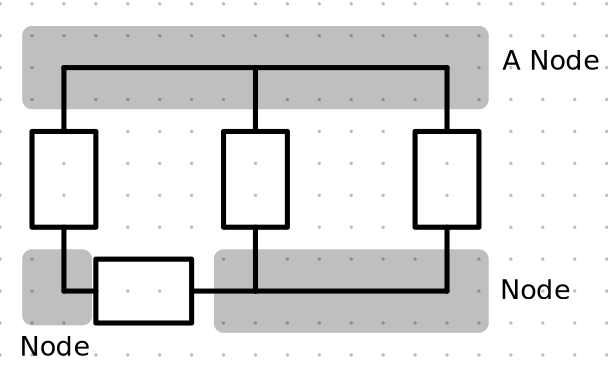
\includegraphics[width=0.5\linewidth]{nodes}
	\end{center}
	
	A series connection is when 2 elements share a single node. The current is the same.
	
	A parallel connection is when there are 2 terminals shared between 2 or more elements. If 2 elements are in parallell (//), then they must both share a node on each side of the elements. 
	\begin{center}
		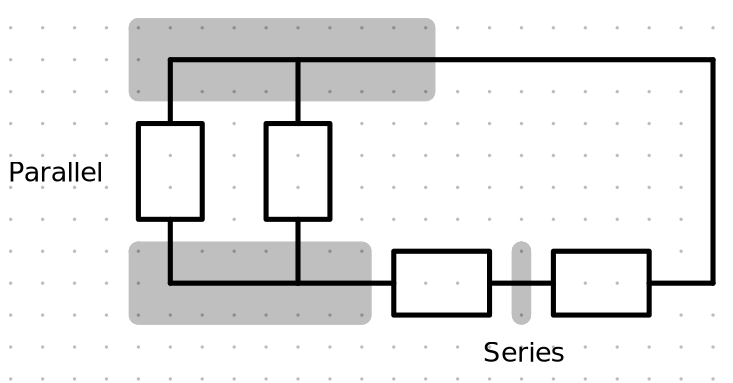
\includegraphics[width=0.5\linewidth]{parallelseries}
	\end{center}
	
	\subsection{Ohms Law}
	Ohms law relates resistance to current and voltage. 
	\begin{align*}
		v=iR
	\end{align*}

	\begin{mdframed}[]
	\textbf{Ex.} Find the current i through the voltage source.
	\begin{center}
		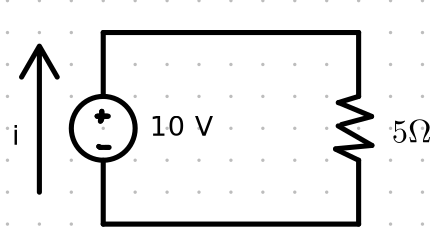
\includegraphics[width=0.35\linewidth]{ex1}
	\end{center}
	We cannot use Ohms law directly since we do not know the resistance of the source.
	
	However, we know that the source and resistance are in parallel, so the voltage at the resistor is also 10 V. We know that it is also in series with the 10 V source, so the current everywhere is the same. 
	\begin{align*}
		v=iR \implies i=\frac{v}{R} = \frac{10}{5} = 2A
	\end{align*}
	Therefore the current in the resistor is 2A, so the current in the source is 2A.
	
	\end{mdframed}
	
	\subsection{KCL (Kirchoffs Current Law)}
	This states that the sum of al currents at any node is 0.
	
	\subsection{KVL (Kirchoffs Voltage Law)}
	This states that the sum of voltages in any loop is 0.
	\begin{center}
		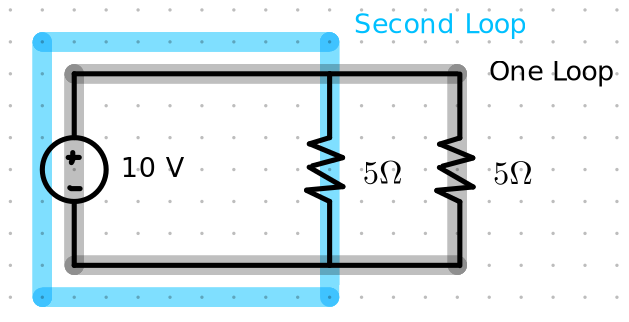
\includegraphics[width=0.4\linewidth]{loop}
	\end{center}
	
	
	So we go around a loop, getting the voltages of each element (recall v=iR) and then solve. We can create multiple KVLs to get a system of equations.
	
	\subsection{Voltage Divider}
	If we have a voltage that goes through 2 resistors in series, the voltage gets divided between both of them.
	\begin{align*}
		v_1 = \frac{R_1}{R_1 + R_2} v_t
	\end{align*} 
	where $v_t$ is the total voltage going in.
	\begin{center}
		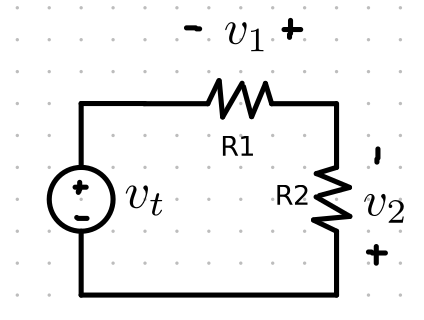
\includegraphics[width=0.3\linewidth]{voltagediv}
	\end{center}
	
	
	\subsection{Current Divider}
	If we have current that goes though 2 resistors in parallel, the current gets divided between both of them. 
	\begin{align*}
		i_1 = \frac{R_2}{R_2+R_1}i_t
	\end{align*}
	where $i_t$ is the total current going in.
	\begin{center}
		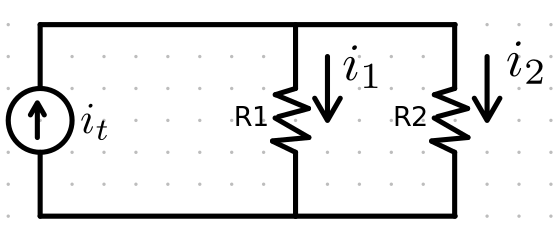
\includegraphics[width=0.4\linewidth]{currentdiv}
	\end{center}

	\subsection{Power}
	If the power is \textbf{positive}, an element \textbf{consumes }power. 
	
	If the power is \textbf{negative}, an element \textbf{produces }power.
	
	We say that:
	\begin{align*}
		P=vi
	\end{align*}

	The net power in a circuit is always 0.
	
	\section{Methods to Analyse Resistive Circuits}
	These methods are ways to easily find all values in a circuit no matter the complexity. 
	
	\subsection{Node Voltage Analysis (NVA)}
	With this method, we need a reference node (Ground node). This node can usually be any node.
	
	This method works on using KCL at each node of the circuit, and then we will get all the currents in terms of node voltage, and then solve the system of equations. 
	\begin{enumerate}[noitemsep]
		\item Identify the number of nodes in the circuit and designate the reference node
		\item If there is an independant voltage source that is not connected to ground, make that a supernode and get it an equation. 
		\item Write the node voltage KCLs for all nodes. Note that if the node is a voltage source connected to ground, we know the voltage. 
		\item Solve the KCLs to get all voltages.
		\item Get the information we need
	\end{enumerate}

	\begin{mdframed}[]
	\textbf{Ex.} Find the node voltages in this circuit. 
	\begin{center}
		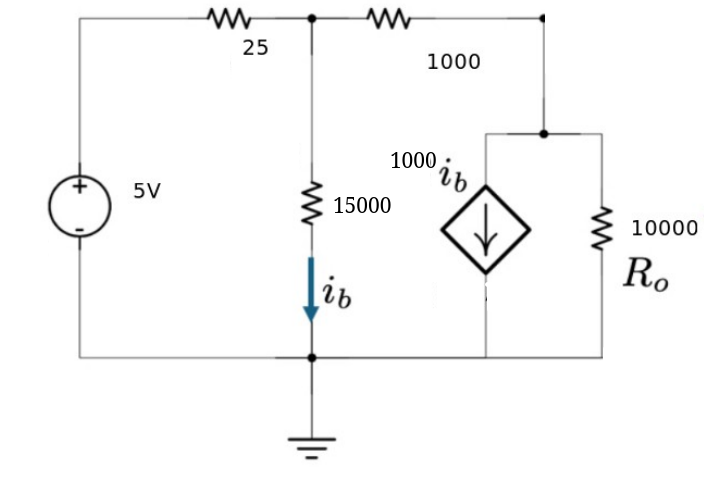
\includegraphics[width=0.5\linewidth]{ex2}
	\end{center}

	We already have a ground. We notice that there is an independant source in this circuit, as well as 3 nodes. 
	
	I will draw in the nodes as well as the current directions I assume (it does not matter what I assume as long as I am consistent).
	
	Note that the leftmost node is 5v. 
	\begin{center}
		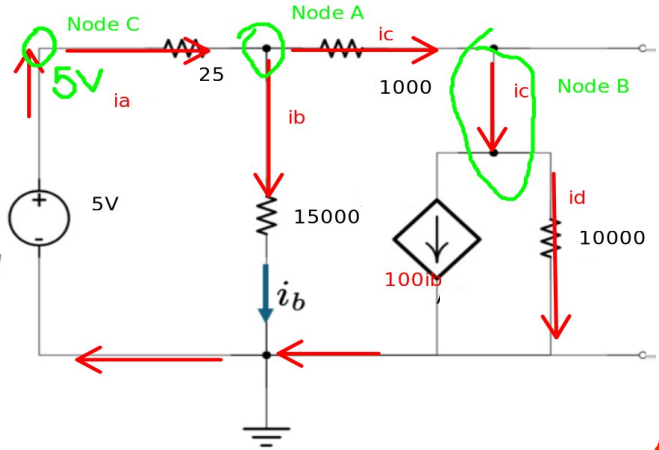
\includegraphics[width=0.5\linewidth]{ex2-2}
	\end{center}
	Now I create equations for nodes A and B. We use the vact that $i=\frac{V}{R}$.
	
	For A: 
	\begin{align*}
		\text{currentIn}=\text{currentOut} \implies \frac{5-V_A}{25} = \frac{V_A}{15000} + \frac{V_A-V_B}{1000}
	\end{align*}

	For B it is a bit harder since we do not know the dependant source, except we actually do since $i_b = \frac{V_A}{15000}$.
	\begin{align*}
		\text{currentIn}=\text{currentOut} \implies \frac{V_A-V_B}{1000} = 100\cdot \frac{V_A}{15000} + \frac{V_B}{10000}
	\end{align*}

	Now I have 2 equations and 2 unknowns so I solve to get $V_A=4.33, V_B=-22.3$. 
	
	\end{mdframed}
	
	\subsection{Mesh Current Analysis (MCA)}
	With this method, we use meshes (loops) in a circuit and do the KVL around those loops. Same idea as the NVA. 
	
	\begin{enumerate}[noitemsep]
		\item Divide the circuit into meshes and assign each mesh a name.
		\item If there is an independant current source common to 2 meshes, form a supermesh and get it an equation. 
		\item Write the mesh current KVLs for all meshes. Note that if there is an independant current source only common to 1 mesh, we know that meshes current.
		\item Solve the KVLs to get all currents.
		\item Get the information we need. 
	\end{enumerate}

	\begin{mdframed}
		\textbf{Ex. } Example found in Module 5.2
	\end{mdframed}
	
	\section{Circuit Theorums}
	These are things that help make a circuit simpler. 
	
	\subsection{Source Transformations}
	We can turn a voltage source and resistor in series into a current source and resistor in parallel.
	
	We can turn a current source and resistor in parallel to a voltage source and resistor in series.
	
	For both of these we just use Ohms law. 
	\begin{center}
		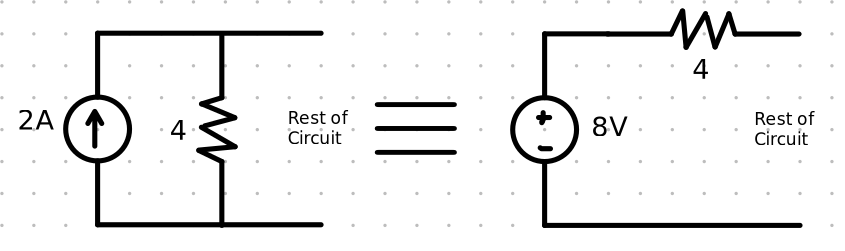
\includegraphics[width=0.7\linewidth]{transSource}
	\end{center}
	
	\subsection{Superposition}
	This states that if we have 2 circuits with current and voltage sources only, then the value of any current or voltage can be gotten by adding the values obtained from each individual source with other sources deactivated.
	
	Deactivating means replace a voltage source with a short circuit (SC), and a current source with an open circuit (OC).
	\begin{center}
		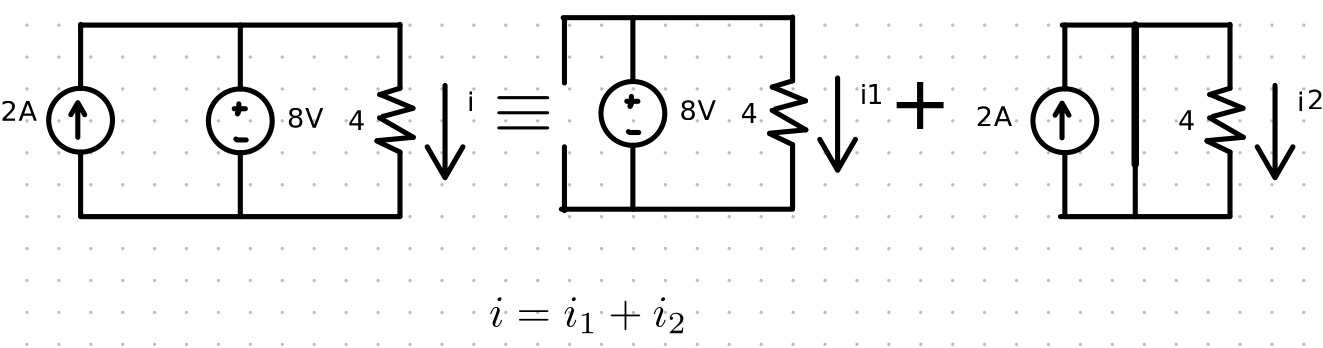
\includegraphics[width=0.9\linewidth]{superposition}
	\end{center}
	
	\subsection{Thevanin}
	Any circuit \textbf{connected between 2 terminals} can be simplified down to an independant voltage source in series with a resistor. 
	
	This voltage source is called the Open Circuit Voltage ($V_{OC}$) and the resistance is called the Thevanin resistance ($R_t$)
	
	To find $V_{OC}$ between 2 terminals, we create an open circuit between those 2 terminals and solve for the voltage across them. This is the $V_{OC}$.
	
	To find $R_t$, we can deactivate all independant sources (Voltage becomes SC, Current becomes OC), then if there are no dependant sources, combine resistors until we have one left. If there are still dependant sources, then we connect a dependant current source with 1A to the terminals, then find the voltage across the terminals, then find $R_t$ knowing 1A current, and voltage. 
	
	\subsection{Norton}
	Any circuit \textbf{connected between 2 terminals} can be simplified down to an independant current source in parallel with a resistor. 
	
	This current source is called the Short Circuit Current ($I_{SC}$) and same as the Thevanin circuit, the resistance is $R_t$.
	
	To find $I_{SC}$ between 2 terminals, we create a short circuit between the terminals and find the current flowing through that wire. This is the $I_{SC}$.
	
	If we know both $I_{SC}$ and $V_{OC}$, then we can find $R_t = \frac{V_{OC}}{I_{SC}}$
	
	\section{Energy Storage Elements}
	
	\subsection{Capacitors and Inductors}
	\textbf{Capacitors and Inductors} are circuit elements that we usually work with in the complex domain. For this module though, we only work in the real domain. 
	
	A capacitor has a \textbf{capacitance C} which is measured in Farads, and an inductor has an \textbf{inductance L} measured in Henrys. 
	
	The current and voltage through a capacitor is:
	\begin{align*}
		i(t)=C\frac{\mathrm{d}V}{\mathrm{d}t}\qquad v(t)=v(t_0) + \frac{1}{C}\int^t_{t_0} i(\tau) \mathrm{d}\tau
	\end{align*}
	
	The current and voltage through an inductor is: 
	\begin{align*}
		v(t)=L\frac{\mathrm{d}i}{\mathrm{d}t}\qquad i(t)=i(t_0) + \frac{1}{L}\int^t_{t_0} v(\tau) \mathrm{d}\tau
	\end{align*}

	\textbf{Inductors} are added together similar to \textbf{resistors} (sum in series, inverse sum in //) while \textbf{capacitors} are added together the \textbf{opposite of resistors }(sum in //, inverse sum in series).
	
	The current in the inductor and voltage in the capacitor can \textbf{never} change instantly.
	
	\subsection{Switches and Initial Conditions}
	A \textbf{switching circuit} has a switch that changes at a certain time. We say that before the switch changes, the circuit has been \textbf{stable} for a very long time (infinity).
	
	When working with switching circuits, we use the following procedure:
	\begin{enumerate}[noitemsep]
		\item Before the switch changes
		\subitem Capacitor is an \textbf{open circuit }and inductor is a \textbf{short circuit}
		\subitem Find the voltage across the capacitor or/and the current through the inductor.
		\item Right after the switch changes
		\subitem Voltage across the capacitor and current in inductor are the same as before.
		\subitem Solve for what we need treating the capacitor as voltage source and inductor as current source.
		\item (Optional) At time is infinity, consider capacitor as open circuit, and inductor as closed circuit. 
	\end{enumerate}

	\begin{mdframed}[]
	\textbf{Ex. } Find $v_1(t^+), v_1(t^-)$ in the following circuit.
	\begin{center}
		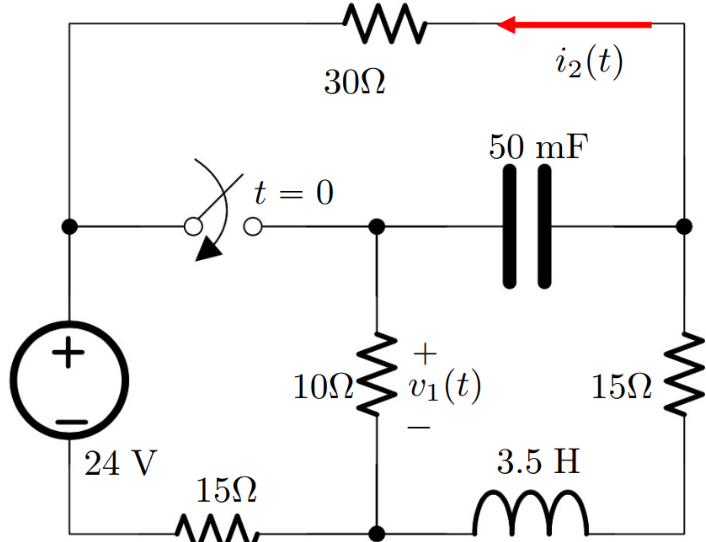
\includegraphics[width=0.45\linewidth]{ex3}
	\end{center}
	When looking before the switch is closed, we draw the capacitor as an OC and indurcot as SC.
	\begin{center}
		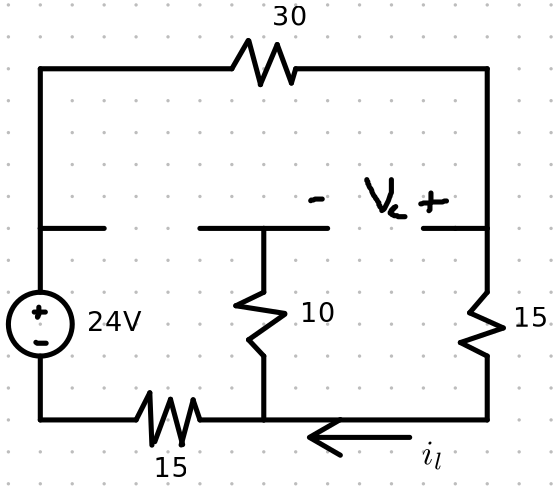
\includegraphics[width=0.3\linewidth]{ex3-2}
	\end{center}
	We can cancel out the 10 $\Omega$ resistor since only one side is connected. This means that the voltage across is is 0. $v_1(0^-)=0$.
	
	The voltage across the capacitor is the same as the voltage across the 15 $\Omega$ resistor.
	
	So I will do a KVL across the whole loop: $-24+30i+15i +15i \implies i=0.4 A$
	
	Then I will use Ohms law to get the voltage across the 15 Ohm resistor: $v=14\cdot 0.4=6$
	
	So we know that $v_c(0^-)=v_c(0^+)=6V$
	
	Also the current in the inductor is: $i_l(t^-)=i_l(t^+)=0.4A$
	
	Now we look at the circuit after the switch is clicked. 
	\begin{center}
		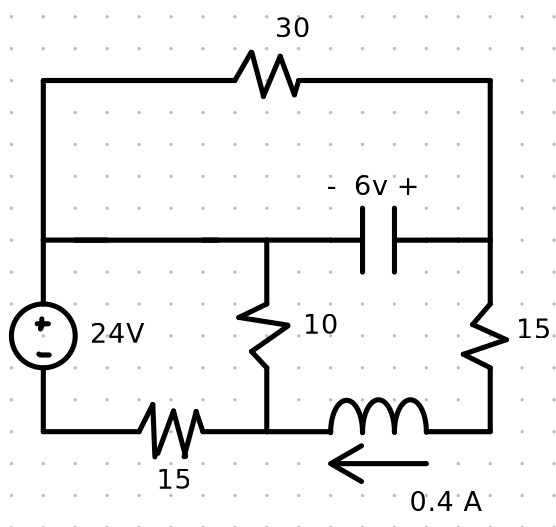
\includegraphics[width=0.3\linewidth]{ex3-3}
	\end{center}

	Now this is a simple circuit if we consider the cap a voltage source, and the inductor a current source. I will use the mesh current analysis to solve. 
	\begin{center}
		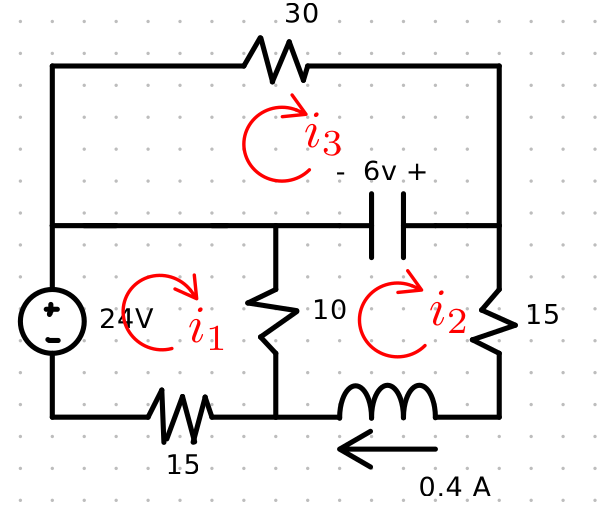
\includegraphics[width=0.3\linewidth]{ex3-4}
	\end{center}
	We know that i2 is 0.4A due to the current source in that mesh.
	
	Do a KVL for mesh 1.
	\begin{align*}
		-24+10(i_1-0.4)+15i_1 = 0 \implies i_1 = 1.12 A
	\end{align*}
	Do a KVL for mesh 2.
	\begin{align*}
		30i_3+6=0 \implies i_3 = -0.2
	\end{align*}
	
	Now that we know the currents, we can find the voltage across the 10 Ohm resistor is just $V=iR=(i_2-i_1)10=7.2 V$
	
	The circuit was verified using multisim as found in Appendix B.
	\end{mdframed}
	
	\section{Complete Responce of RL and RC}
	This module is very similar to module 5 except we find the v(t) or i(t) for any t using an equation. 
	
	We follow the same steps of: 
	\begin{enumerate}[noitemsep]
		\item \textbf{Before} the switch changes
		\subitem Capacitor is an \textbf{open circuit }and inductor is a \textbf{short circuit}
		\subitem Find the voltage across the capacitor or/and the current through the inductor.
		\item \textbf{Right after} the switch changes
		\subitem Voltage across the capacitor and current in inductor are the same as before.
		\subitem Solve for Norton and Thevanin circuits treating the capacitor as voltage source and inductor as current source.
		\item Sub values into the current or voltage in inductor or capacitor equation.
	\end{enumerate}
	
	\subsection{RC Circuits (Resistance and Capacitor)}
	We use the formula:
	\begin{align*}
		v_c(t)=V_{OC}+(v_c(0^+)-V_{OC})e^{-\frac{t}{R_tC}}
	\end{align*}
	
	\subsection{RL Circuits (Resistor and Inductor)}
	We use the formula:
	\begin{align*}
		i_l(t)=I_{SC}+(i_l(0^+)-I_{SC})e^{-\frac{tR_t}{L}}
	\end{align*}

	\subsection{Multiple Periods}
	We can have \textbf{multiple periods where we need a different equation.}
	
	This is very simple in that there is a seperate $I_{SC}$ or $V_{OC}$ for each time period, and the initial part ($v_c(0^+)$ or $i_l(0^+)$) is just the final of the previous time period. 
	
	\section{AC Analysis of RLC Circuits using Phasors}
	When working in the complex domain, we say we are working in the \textbf{phasor domain or frequency domain}. 
	
	We are given the voltage source as a sinusoidial in the form of $v(t)=A\cos(\omega t+\phi)$ where A is the amplitude of the voltage, $\omega$ is the period, and $\phi$ is the phase angle. We can also write this in \textbf{phasor form} as $v(t)=A\angle \phi$
	
	To work in the phasor domain, we do the following steps:
	\begin{enumerate}[noitemsep]
		\item Represent all independant sources in their phasor form.
		\item Represent all unknown currents and voltages as phasors (Inductors, Capacitors, Resistors, etc.)
		\item Treat the circuit as a convential circuit and solve using conventional means such as KVL, KCL, Source Transformations, NVA, etc. 
		\item Once we have the piece of information we want, \textbf{put it back into the time domain.}
	\end{enumerate}

	\subsection{Inductance}

	In the phasor domain, resistors still are measured in Ohms. We do not have to change anything. 
	
	Capacitors need to be converted into their \textbf{impedance} (complex form of resistance) using the equation: 
	\begin{align*}
		Z=\frac{1}{\jmath\omega C}\Omega = \frac{-\jmath}{\omega C}\Omega
	\end{align*}

	Inductors also have to be converted into their \textbf{impedance} using the equation:
	\begin{align*}
		Z=j\omega L \Omega
	\end{align*}
	
	\subsection{Admittance}
	The admittance $Y$ is just the inverse of the impedance $Z$. 
	\begin{align*}
		Y=Z^{-1}=\frac{1}{Z}
	\end{align*}
	
	\section{Power Calculations in AC Circuits}
	This module mostly just has to do with using the correct equations and subbing in the correct values. These equations are located on the formula sheet in Appendix A.
	
	\newpage
	\appendix
	\begin{center}
		\Large\textbf{Appendix} \\
		\vspace{0.5em}
	\end{center}
	
	\section{Formula Sheet}
	\begin{center}
		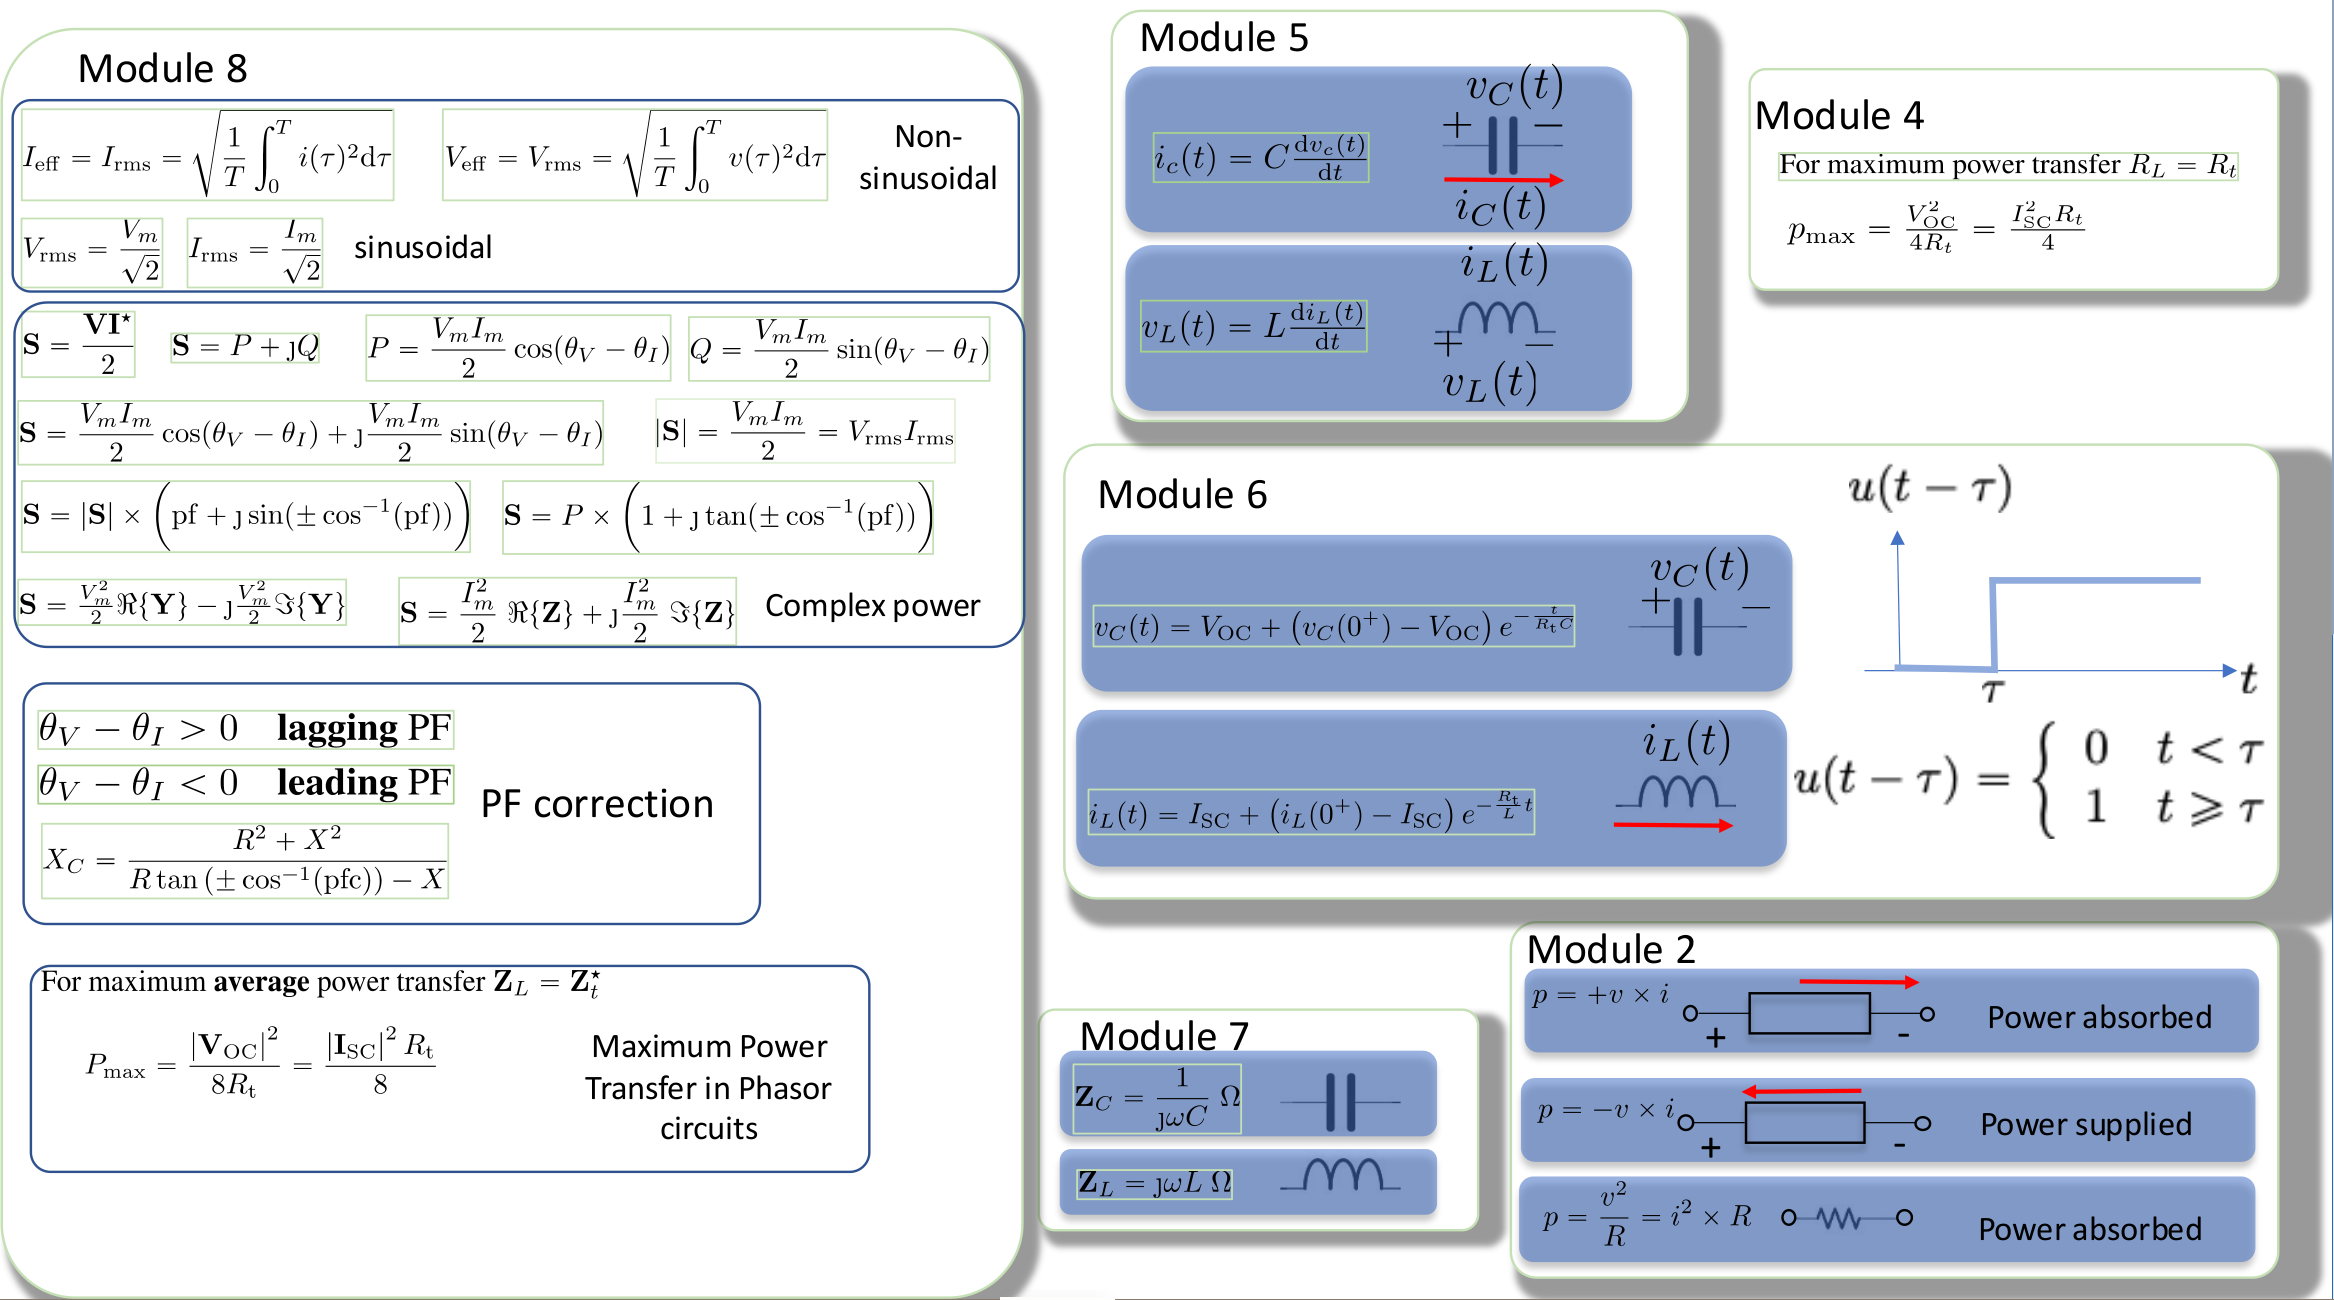
\includegraphics[width=0.99\linewidth]{formulaside1}
	\end{center}
	\begin{center}
		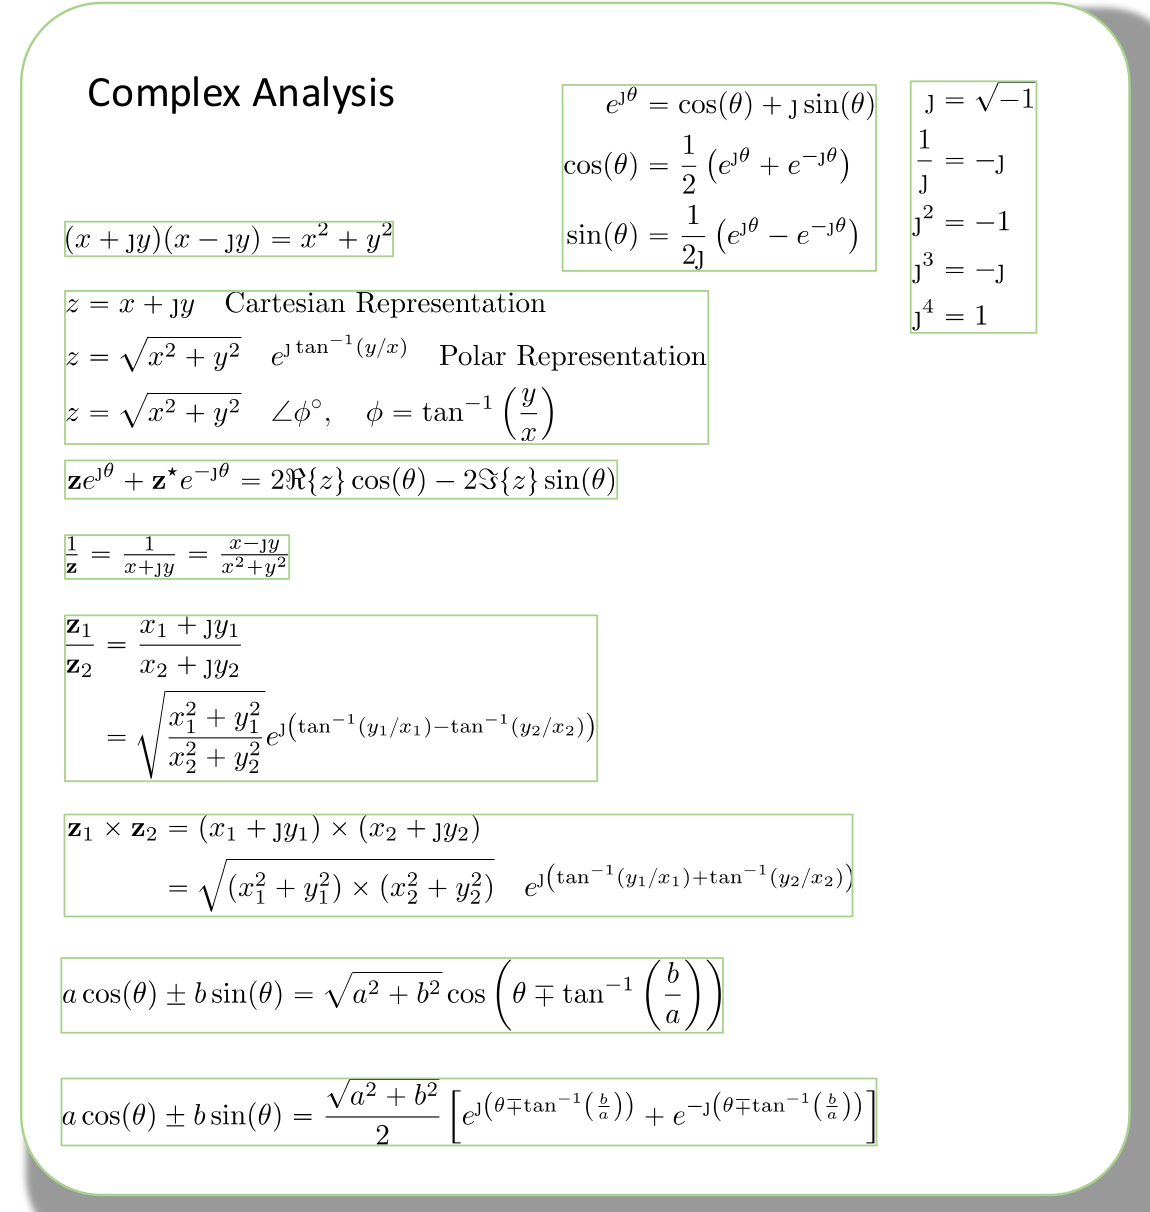
\includegraphics[width=0.5\linewidth]{formulaside2}
	\end{center}
	
	
	\section{Multisim Verification for 5.2}
	\begin{center}
		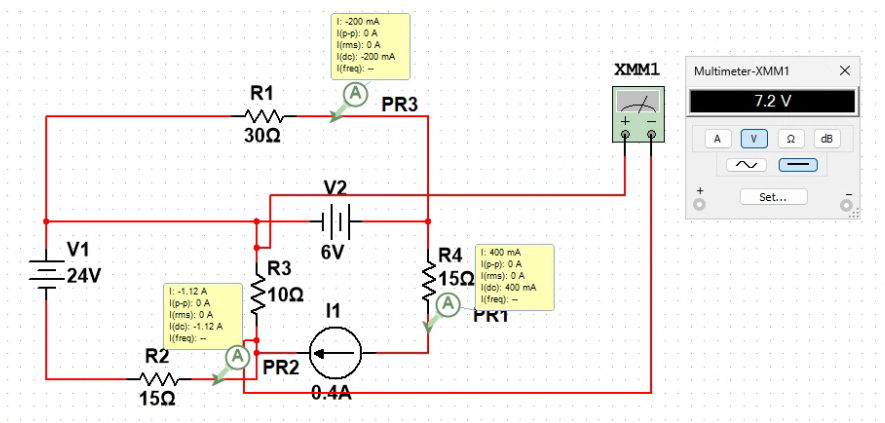
\includegraphics[width=0.8\linewidth]{ex3-5}
	\end{center}
	
	
	
	
\end{document}